\label{chapter:Installation}
\index{Installation}
The first step in the software installation process is to obtain the \mut\ examples, executables and database files from
\github.  To do this:
\begin{itemize}
     \item Click on this link, \url{https://github.com/Grdbldr/MUT_Examples.git}, which will take you the \mut\_Examples \github\ page.
     \item Click on the green 'Code' button.

        \includegraphics[width=0.97\textwidth]{2_1_github_codebutton}

     \item Choose 'Download ZIP' from the drop-down menu.

        \includegraphics[width=0.5\textwidth]{2_2_github_downloadzip}

\end{itemize}

Once the download is complete, the zip file can be found in the \windows\ Downloads folder.  The contents need to be extracted to a local directory by right-clicking on the download file and choosing 'Extract All...' from the drop-down menu:

        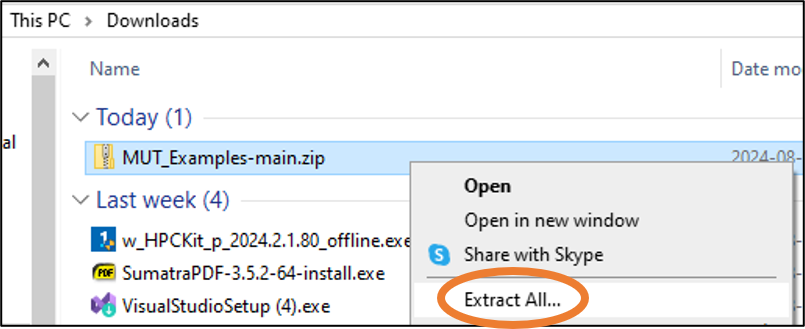
\includegraphics[width=0.6\textwidth]{2_2b_ExtractAll.png}

This opens the Extract dialogue, where you are free to choose a different drive and folder to store the extracted files.  Here we changed the destination folder to \verb+C:\MUT+.  Click the 'Extract' button:

        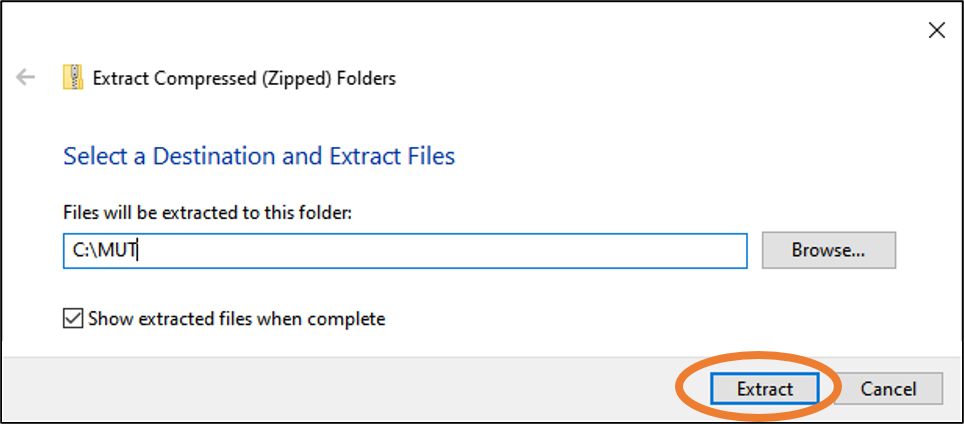
\includegraphics[width=0.6\textwidth]{2_2c_ExtractAllToMUT.png}

The extracted contents can now be found in the specified destination folder:

        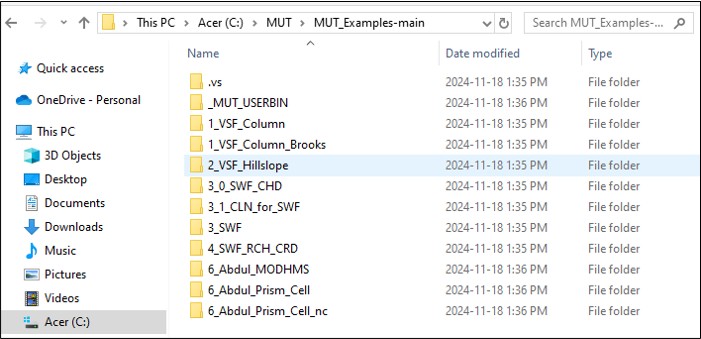
\includegraphics[width=0.8\textwidth]{2_2d_DestFolder.png}

This folder contains a subfolder called \texttt{\_MUT\_USERBIN}, which contains the following files:


        \includegraphics[width=0.8\textwidth]{2_2e_Mut_UserBin.png} \label{page:userbin}
        \phantomsection\label{page:userbin}.


These include the executable and supporting files for \mut\ and the executable for \mfus.

Before you run \mut\ for the first time, you need to define a windows environment variable called \bin, which contains the path to the \texttt{\_MUT\_USERBIN} folder, and modify the existing \texttt{PATH} variable.

First,  highlight the path by clicking on it in the File Explorer window, then copy it by pressing CTRL-C or by right-clicking and choosing 'Copy' from the drop-down menu, as shown here:

        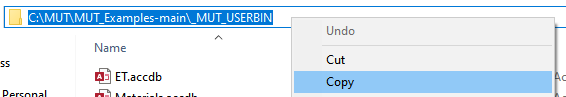
\includegraphics[width=0.8\textwidth]{2_2f_CopyMut_userbinPpath}


To define the environment variables:
\begin{itemize}
     \item Type the string 'en' in the windows taskbar search field and open the 'Edit the system environment variables' dialogue:

        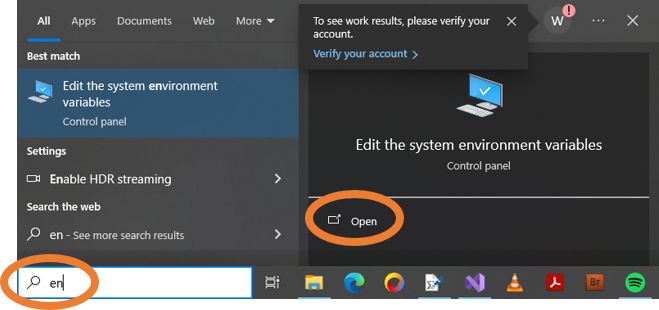
\includegraphics[width=0.6\textwidth]{2_3_EnvVar}

     \item Click on the 'Environment variables...' button at the bottom of the dialogue:

        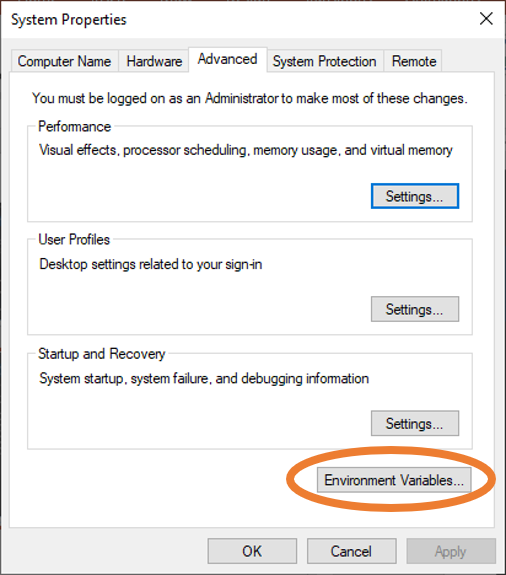
\includegraphics[width=0.4\textwidth]{2_4_EnvVar}


     \item Click on the 'New' button:

        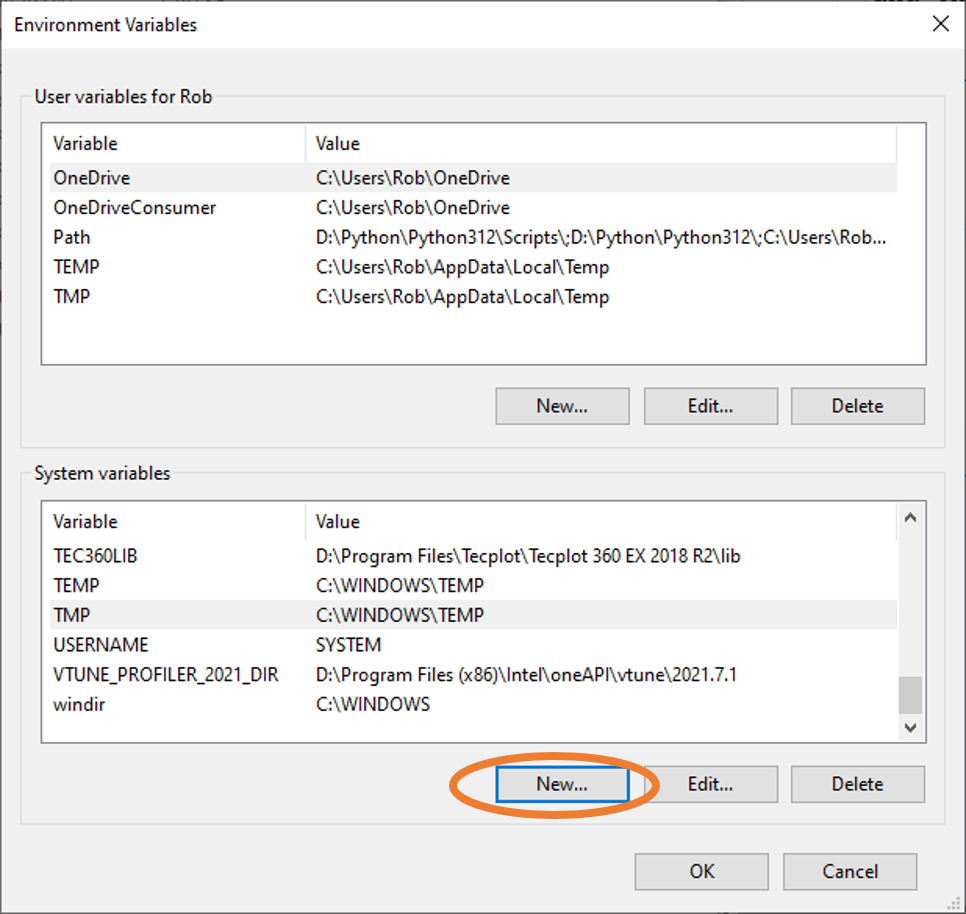
\includegraphics[width=0.4\textwidth]{2_5_EnvVarNewButton}

     \item Add a new variable named \bin\ and define the variable value by pasting in the path copied earlier, then click the 'OK' button:

        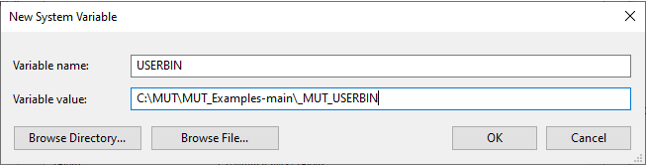
\includegraphics[width=0.4\textwidth]{2_6_EnvVarUserBin}

     \item Add the path to \bin\ to the existing \texttt{Path} variable.  First, choose \texttt{Path}, then click the 'Edit...' button:

        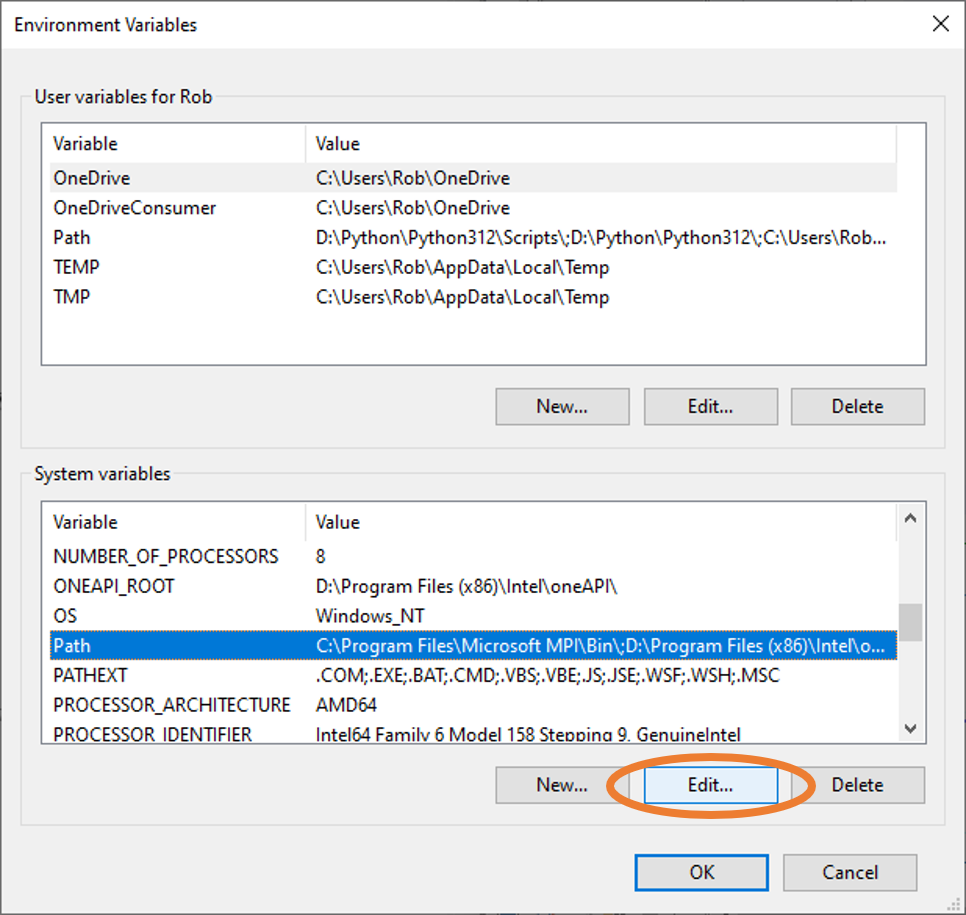
\includegraphics[width=0.4\textwidth]{2_7_EnvVarEditPath}

     \item Click the 'New' button and paste in the path copied earlier, then click the 'OK' button:

        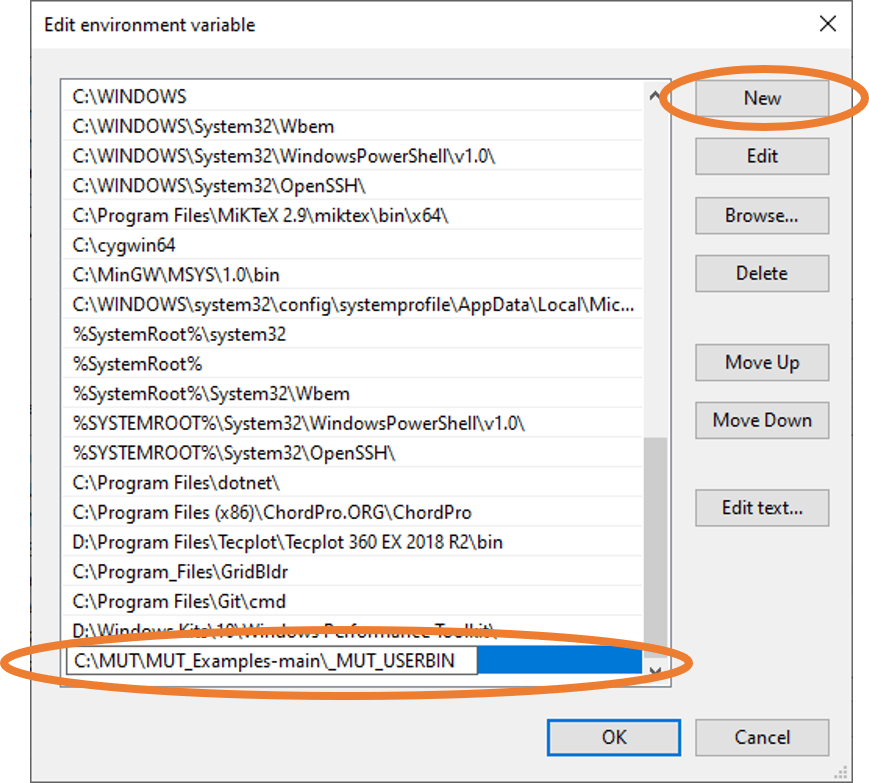
\includegraphics[width=0.4\textwidth]{2_8_EnvVarNewPath}

\end{itemize}

You should now be able to run \mut\ and \mfus\ from the command prompt.  To test this, start a new command prompt, then type \texttt{mut}, you should see the \mut\ header:

    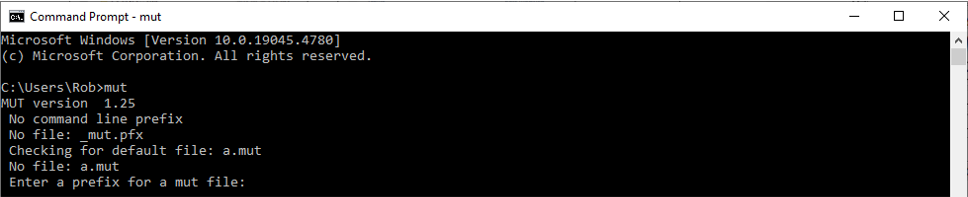
\includegraphics[width=0.95\textwidth]{2_9_mutheader}

Type \texttt{ctrl-C} to stop the program.

Run \mfus\ by typing \texttt{usgs\_1}.  You should see the \mfus\ header:

    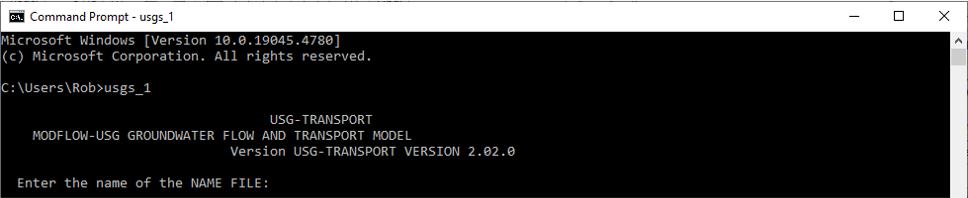
\includegraphics[width=0.95\textwidth]{2_10_mfusheader}

Type \texttt{ctrl-C} to stop the program.

If this is not the case, check the definitions of the \bin\ and PATH variables.  If they are correct, you may need to re-boot your computer and try again.

A licensed version of \tecplot\ can be obtained from \url{https://tecplot.com/products/tecplot-360/}.  They have a free 30-day trial option for those who want to assess the software before purchase.  They also offer educational discounts.

Those of you who are just interested in running the \mut\ and \mfus\ programs have completed the required  software installation tasks and can proceed to Chapter~\ref{chapter:ModelBuild}, \textbf{Model Build}.

Those who want to view and possibly modify and re-compile the source code for \mut\ and \mfus\ should proceed with these instructions for setting up your \windows\ programming environment.

As was stated earlier, we use and recommend \vstudio\ and \ifort. You should install \vstudio\ before \ifort, which will then be automatically integrated into \vstudio.

A free version of the latest \vstudio\ (currently 2022) can be obtained from \url{https://visualstudio.microsoft.com/vs/community/}. Once you are on the site just click the \texttt{Download} button.  This will download a file (e.g.\ \texttt{VisualStudioSetup.exe}) which can be run to install \vstudio.  If you already have a version of \vstudio, you can choose to keep your old version and add the latest version.  When you come to the installation options 'Workloads' page, be sure to check the option for \texttt{Desktop development with C++}, shown here:

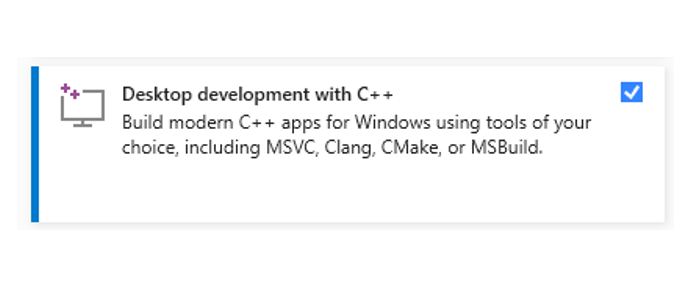
\includegraphics[width=0.6\textwidth]{2_11_vstudiooption}

A free version of the latest \ifort\ compiler can be obtained from \url{https://www.intel.com/content/www/us/en/developer/tools/oneapi/hpc-toolkit.html}.
Once you are on the site just click the \texttt{Get It Now} button to download the Intel® HPC Toolkit, which includes \ifort.  Choose the \texttt{Windows} option then the \texttt{Offline Installer} option. Now you can either fill in the required information and start the download or choose to \texttt{Continue as guest(download starts immediately)}.  This will download a file (e.g.\ \texttt{w\_HPCKit\_p\_2024.2.1.80\_offline.exe}) which can be run to install \ifort.

You can check the installation of \vstudio\ and \ifort\ by starting \vstudio\ and choosing \texttt{Create a new project}.  The window that appears should have  links for creating Fortran projects, as shown here:

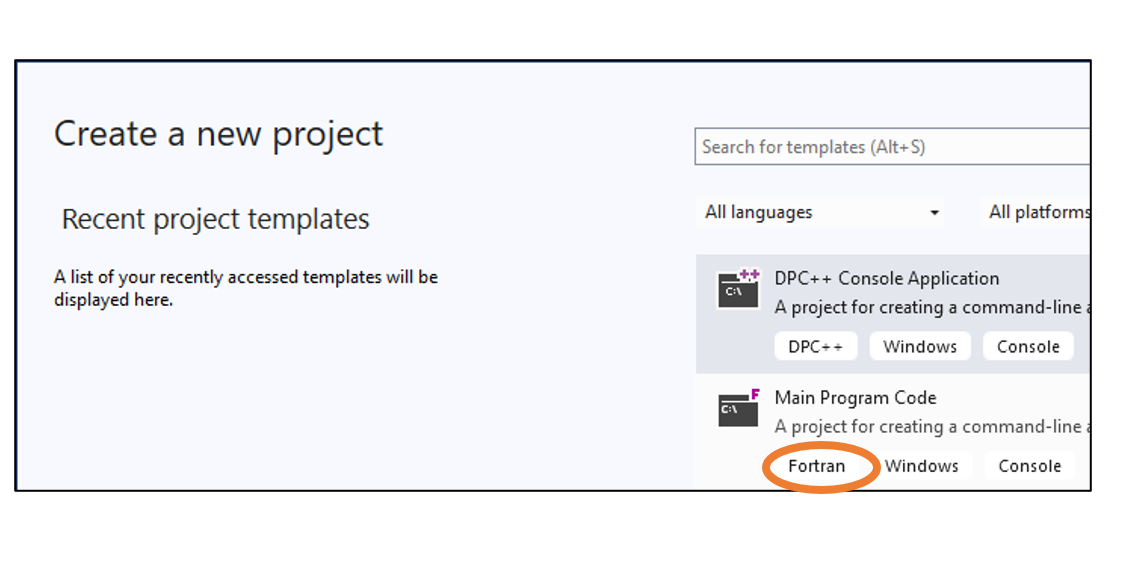
\includegraphics[width=0.8\textwidth]{2_12_createproject}

The \mut\ source files can be obtained from a \github\ repository at \url{https://github.com/Grdbldr/MUT_Source.git}.  Since \github\ has been integrated into \vstudio\, we will use it to download the \mut\ repository.  When you start \vstudio\, choose this option:

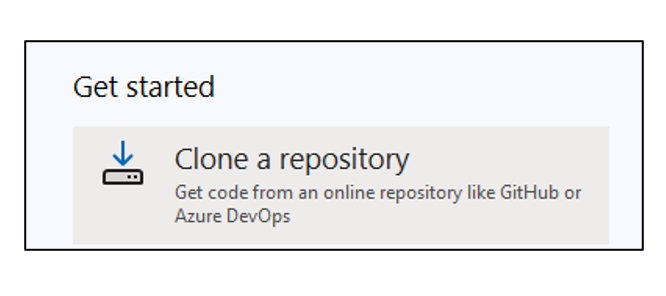
\includegraphics[width=0.4\textwidth]{2_13_clonerepo}

This opens the dialogue box shown below, where you can define the repository location on \github\ and the path to the local repository.  You can copy the link from the PDF file by right-clicking on it and choosing \texttt{Copy Link Adress}.

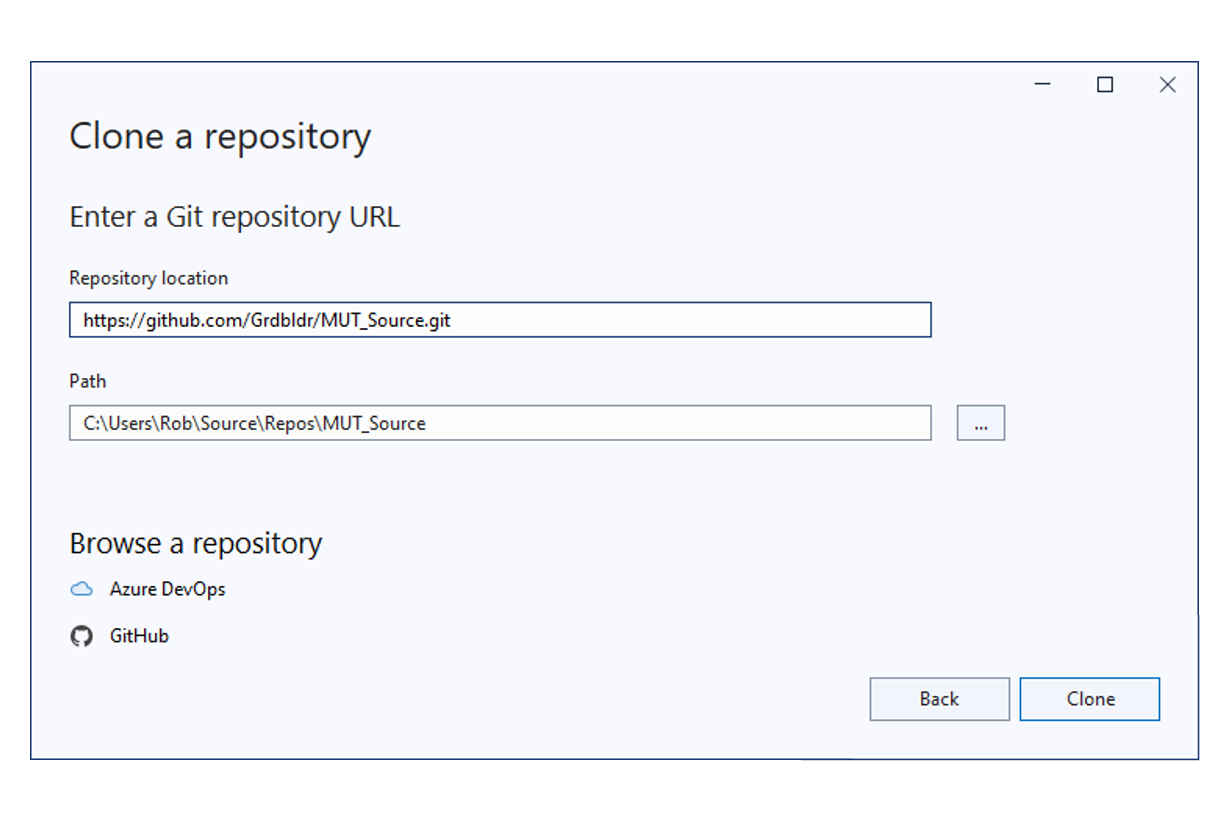
\includegraphics[width=0.7\textwidth]{2_14_clonerepodialogue}

Now choose the \texttt{GitHub} option under \texttt{Browse a Repository} and you will see this dialogue shown below, Choose \texttt{Grdbldr/MUT\_Source} from the list of repositories then click the \texttt{Clone} button.

  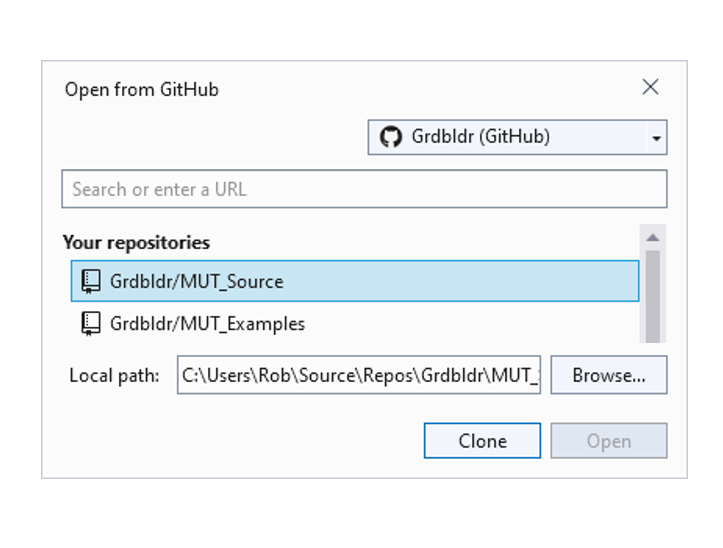
\includegraphics[width=0.45\textwidth]{2_15_clonemutsource}

This shows the \vstudio\ window after \texttt{Grdbldr/MUT\_Source} has been cloned. Note the \github\ window on the right side, and information along the bottom about the project:

    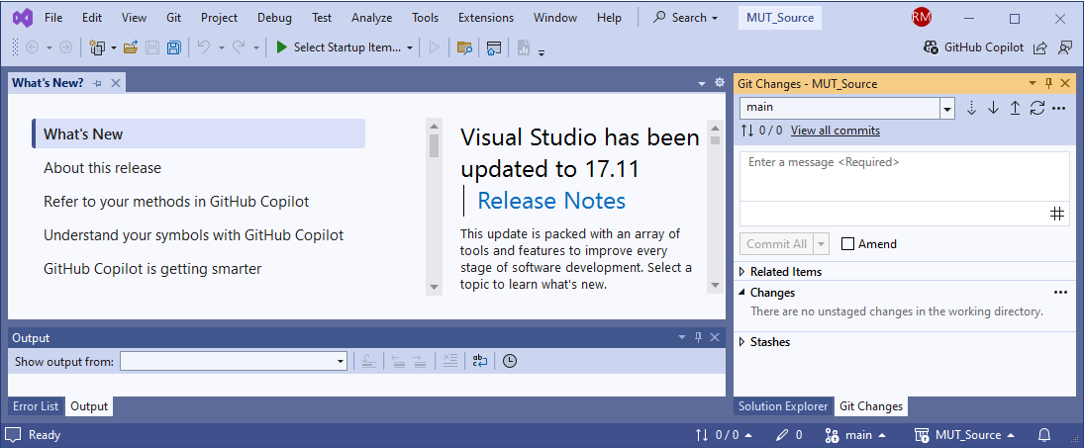
\includegraphics[width=0.7\textwidth]{2_16_vstudiomutsource}

Details about using \github\ in \vstudio\ are given in Tutorial~\ref{tutorial:GitInVStudio}.

The software has been developed and tested under:
\begin{itemize}
    \item Windows 10
    \item \tecplot 360 EX 2018 R2
    \item Microsoft Visual Studio Community 2022, Version 17.11.1
    \item Intel® Fortran Compiler   2024.1
\end{itemize} 